\documentclass[crop,tikz]{standalone}
\usepackage{pgfplots}
\pgfplotsset{compat=1.18}

% Flow inside a 3-dimensional pipe
%
% Let d_1 and d_3 be the constant diameters of the 1st and 3rd pipe
% sections. Let d_2(z) be the diameter of the pipe between sections 1
% and 3 with constant slope. Then the (divergence free) velocity is
% given by
%
% \vec{v}(r,z) = v_0[(d_1/d_2(z))^2\vec{e}_z+d_1^2d_2'(z)r/d_2^3(z)\vec{e}_r]

\usetikzlibrary{arrows.meta}

\pgfplotsset{
  inverted/.style = {
    every axis legend/.append style={
      draw=white,
      fill=hardblack,
      text=white
    }
  },
}

\begin{document}
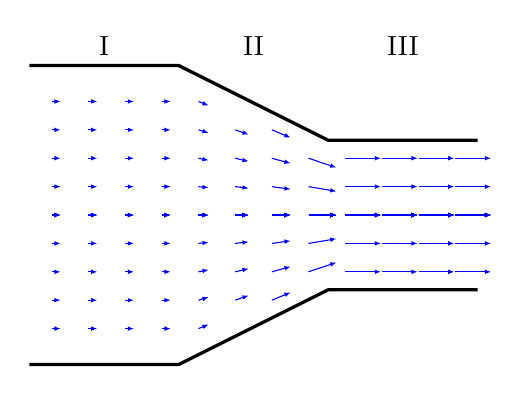
\begin{tikzpicture}
  \pgfmathsetmacro{\Length}{1} % length of each pipe section
  \pgfmathsetmacro{\diamA}{2} % diameter of section 1
  \pgfmathsetmacro{\diamC}{1} % diameter of section 3
  \begin{axis}[
    width={0.6\linewidth},
    view={0}{90},
    axis equal image,
    hide axis,
    xmin=0, xmax={3*\Length},
    ymin={-\diamA/2}, ymax=1.3,
    unbounded coords=discard,
    declare function={
      % diameter at z
      diam(\z) = ifthenelse(\z<\Length, \diamA, ifthenelse(\z<2*\Length, \diamA + (\diamC - \diamA)*(\z/\Length - 1), \diamC));
      % slope of diameter at z
      dprime(\z) = ifthenelse(\z<\Length, 0, ifthenelse(\z<2*\Length, (\diamC - \diamA)/\Length, 0));
      % radius at z
      radius(\z) = 0.5*diam(\z);
      % is inside tube?
      inside(\z,\r) = ifthenelse(abs(\r)<0.92*radius(\z), 1, 0);
      % z component of velocity
      vz(\z,\r) = inside(\z, \r)*(\diamA/diam(\z))^2;
      % radial component of velocity
      vr(\z,\r) = inside(\z, \r)*(\diamA^2*dprime(\z)/diam(\z)^3)*\r;
      % set points outside of pipe to 0/0
      maskr(\z,\r) = ifthenelse(abs(\r)<0.9*radius(\z), \r, 0/0);
    },
    clip=false,
    ]
    \addplot3[
        blue,
        quiver={
            u={vz(x,y)},
            v={vr(x,y)},
            scale arrows=0.06,
        },
        -{Latex[length=0.8mm]},
        domain=0.15:2.85,
        y domain=-0.95:0.95,
        samples=12,
        samples y=11,
    ] (x,{maskr(x,y)},0);
    % pipe
    \draw[black, very thick] (0,{\diamA/2}) -- ({\Length},{\diamA/2}) -- ({2*\Length},{\diamC/2}) -- ({3*\Length},{\diamC/2});
    \draw[black, very thick] (0,{-\diamA/2}) -- ({\Length},{-\diamA/2}) -- ({2*\Length},{-\diamC/2}) -- ({3*\Length},{-\diamC/2});
    % labels
    \node[above] at ({0.5*\Length},{\diamA/2}) {I};
    \node[above] at ({1.5*\Length},{\diamA/2}) {II};
    \node[above] at ({2.5*\Length},{\diamA/2}) {III};
    % separation of pipe sections
    % \draw[gray,dashed,thin] ({\Length},{\diamA/2}) -- ({\Length},{-\diamA/2});
    % \draw[gray,dashed,thin] ({2*\Length},{\diamC/2}) -- ({2*\Length},{-\diamC/2});
  \end{axis}
\end{tikzpicture}
\end{document}
